%!TEX root = ./report.tex
\section{Solution}
\subsection{Practical Info}
Attached to this report you will find a CD containing the following.
\begin{itemize}
  \item The final implementation of the algorithm in C\# souce code that builds against .NET 4.0.
  \item A comma seperated data set of the geographical locations of Pizza Hut, McDonalds and Burger King restaurants in the US.
  \item A parser for the above data set.
  \item An open source implementation of Fortune's algorithm \cite{fortunes}
\end{itemize}

\subsection{Overview}
The solution is based on the description provided in \cite{computational_geometry} of point location and Voronoi diagrams. We do not describe everything in detail here, but refer to \cite{computational_geometry}. Instead we emphasize the steps we took to merge the algorithms, and solve the problems explained in our problem statement. The implementation of the trapezoidal map $T$ and the search tree $D$ is provided by the authors, and here we provide details on the operation that handles the insertion of a segment crossing multiple existing trapezoids. Our main work constitutes the final merged algorithm and its implementation.
\paragraph{}
An obvious way of accomplishing the problem at hand, would be to run the two algorithms sequentially by taking the output from Fortune's algorithm, and feed it directly to the algorithm for the trapezoidal map. Both algorithms run in O(nlogn)  time so the complexity would the same. Instead, we merge the two algorithms by simply extracting the trapezoidal algorithm as a stepwise procedure which we then call in each iteration of Fortune's algorithm. It is easy to see that this does not result in any improvements in terms of complexity as we are virtually doing the same thing.  

\subsection{Point location in Voronoi}
The search tree is implemented with a standard composite pattern, and offers a $FindTrapezoid(point)$ operation that will return the trapezoid containing the query point.  Recall that a trapezoid is simply defined by its side points and top and bottom segment. As each segment is just a segment we got from the Voronoi diagram, it holds a reference to the site of the Voronoi cell and this reference is eventually the only way for that trapezoid to tell which Voronoi cells it lies in. 

\paragraph{}
Each time a segment is discovered in the Voronoi algorithm, it is inserted into the trapezoidal map, and $D$ is updated with new sub trees according to the trapezoids appearing from inserting the new segment. A this point a lot of re-wiring occurs, as new and existing trapezoids need to have their neighbourhoods updated correctly. An example of this is seen in Figure~\ref{fig:contained_segment}. 

\begin{figure}[]
    \centering
      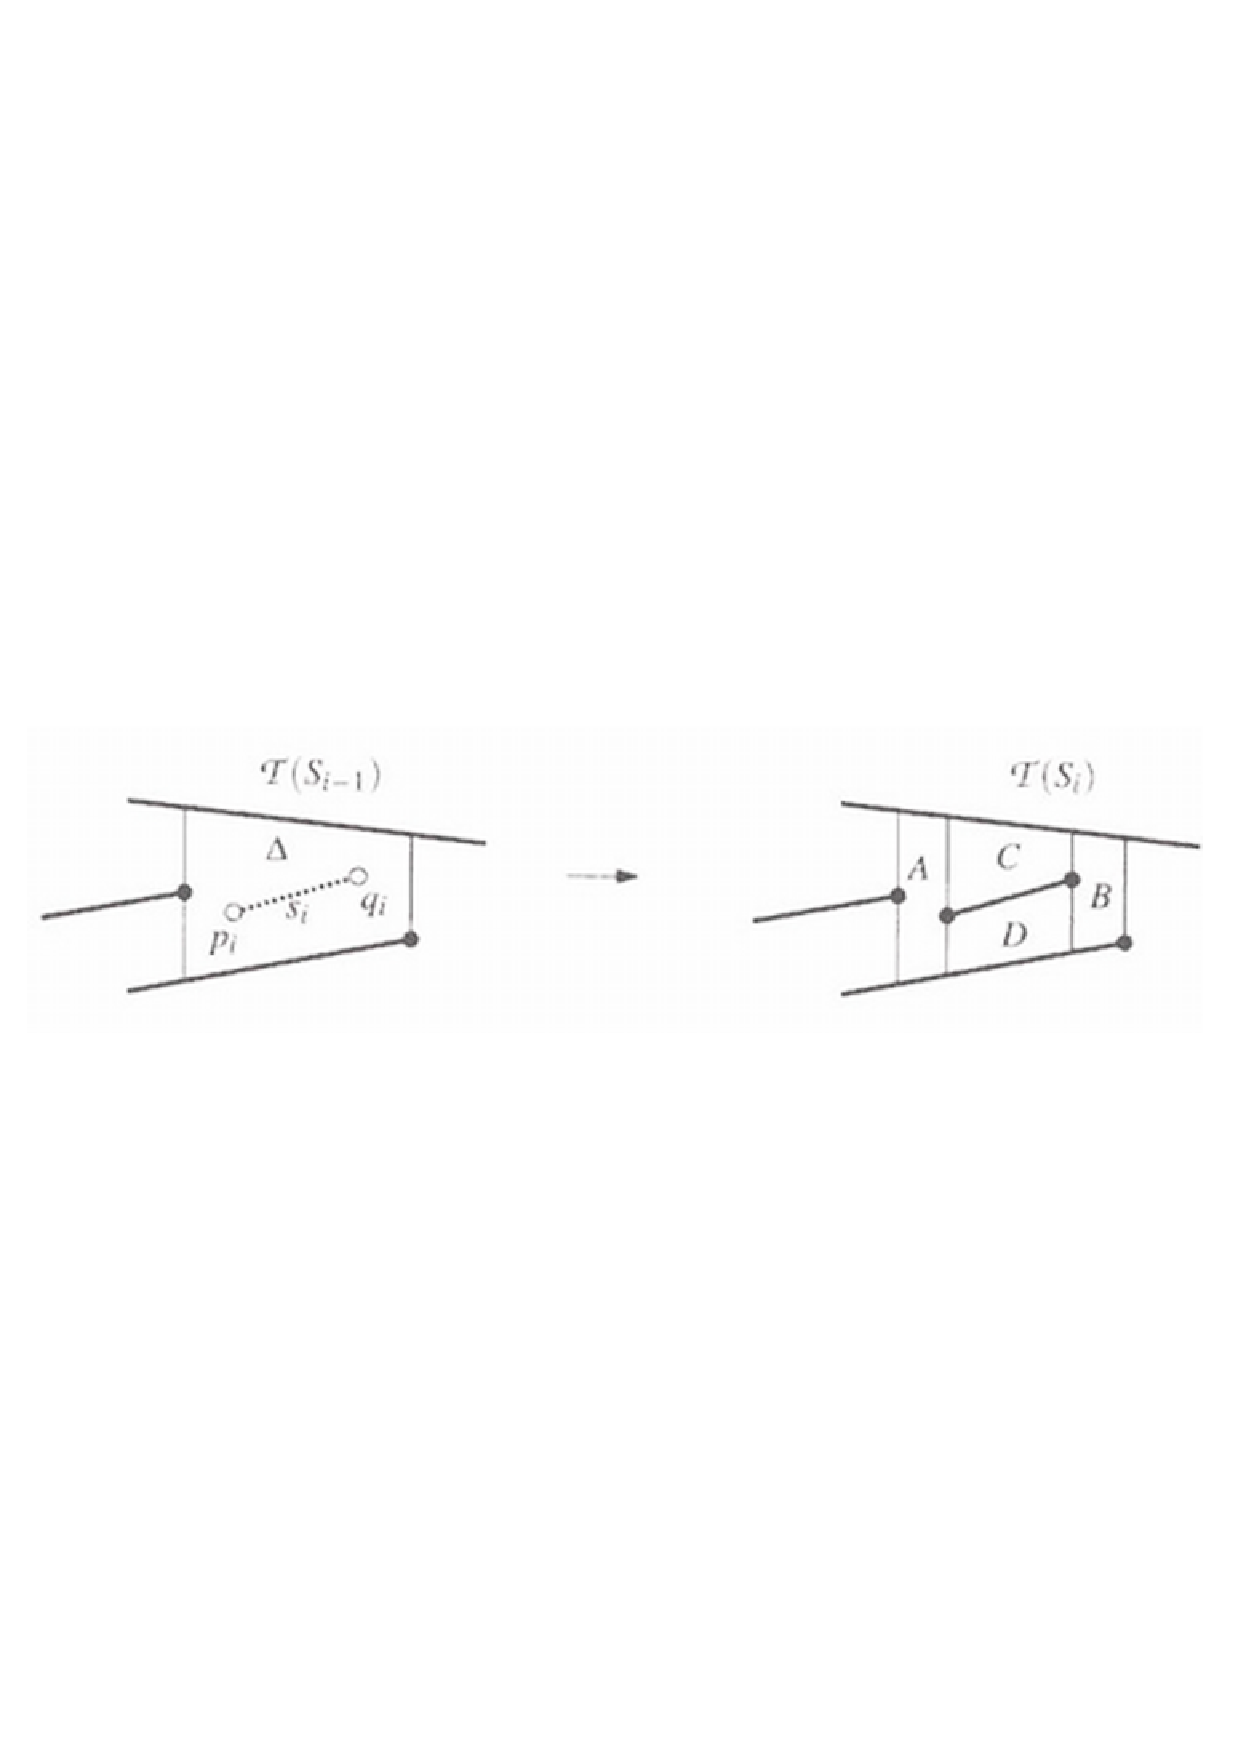
\includegraphics[width=90mm]{images/contained_segment.pdf}
    \caption{Inserting a segment in $T$ that is contained inside a single existing trapezoids}
    \label{fig:contained_segment}
\end{figure}

When the segment is contained in an existing trapezoid we need to make sure that we identify the new trapezoids created from inserting the segment, and update $D$ with a corresponding sub tree. In the case where a new segment crosses several existing trapezoids, things get a bit more tricky, and we will in the following explain how it can be solved. The situation is shown in Figure~\ref{fig:intersecting_segments}.

\begin{figure}[]
    \centering
      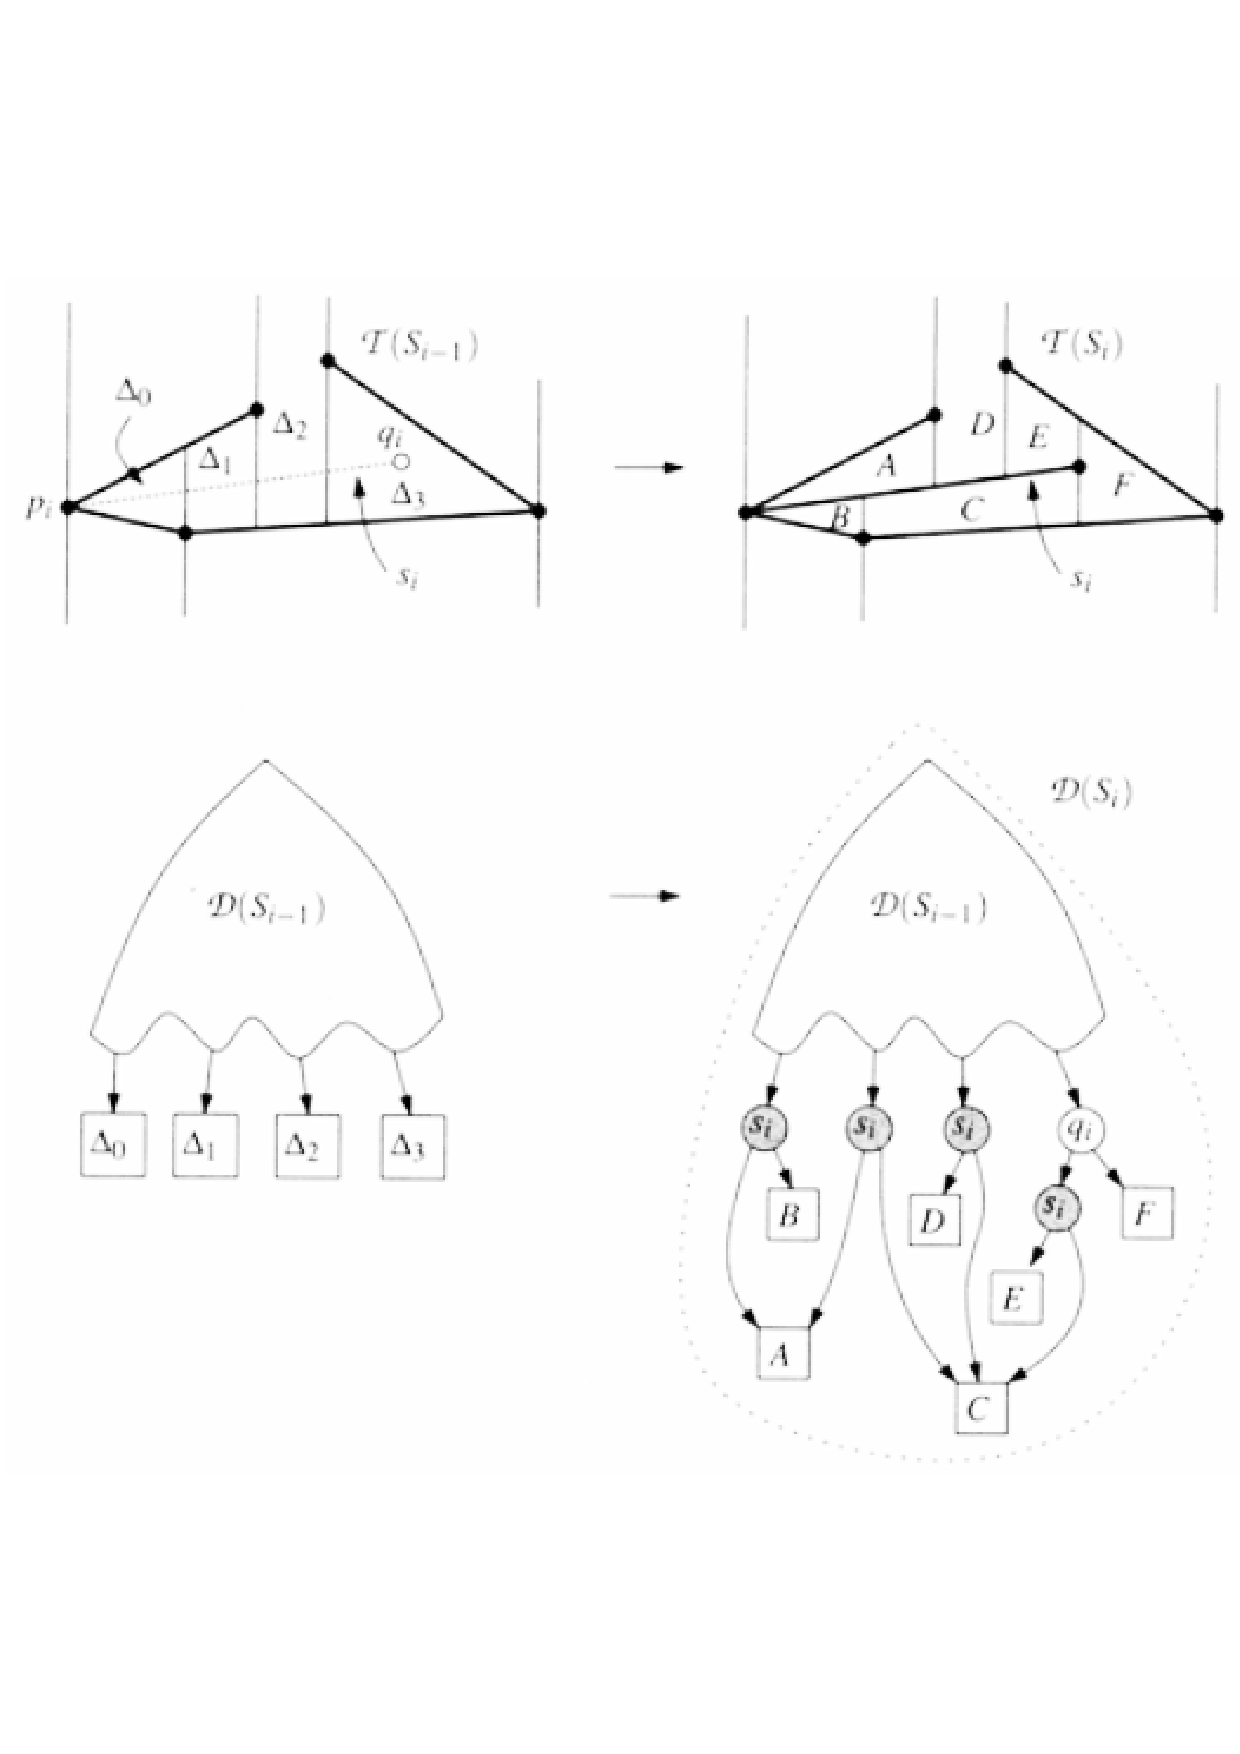
\includegraphics[width=90mm]{images/intersecting_and_tree.pdf}
    \caption{The trapezoidal map and search tree before and after inserting a segment that crosses several trapezoids. Notice how a trapezoid like $C$ can easily end up having multiple parents}
    \label{fig:intersecting_segments}
\end{figure}

\cite{computational_geometry} provides a good high level description of how to handle this situation and states that the whole operation can be done in linear time in the number of involved trapezoids, which is possible because we can find neighbours by following pointers from one trapezoid to the next  - we do not need to look up neighbouring trapezoids in $D$. To handle the different cases of the position of the inserted segment, we first take care of the boundaries when one or both of the new segment's endpoints are connected to existing vertices, which is handled much like the contained case. Secondly, we have to create new trapezoids. As an example, in Figure~\ref{fig:intersecting_segments}, we create a  trapezoid $C$ with a left point from $\Delta 1$, a right point that will be the right most vertex of the newly inserted segment, the top will be the new segment, and the bottom will be the segment shared by  $\Delta 1$,  $\Delta 2$ and  $\Delta 3$.  Our solution to this is to always handle $\Delta 0$ and $\Delta 3$ first in isolation, i.e. adding trapezoids much like with the case of the contained segment, and set the neighbourhoods. Secondly we do a recursive merge of the old trapezoids above the inserted segment, and under the segment. The pseudo code for the upper merge is shown in Algorithm~\ref{alg:MERGEUPPER}.


\IncMargin{1em}
\begin{algorithm}[]
\label{alg:MERGEUPPER}
\SetKwData{Left}{left}\SetKwData{This}{this}\SetKwData{Up}{up}
\SetKwFunction{Union}{Union}\SetKwFunction{FindCompress}{FindCompress}
\SetKwInOut{Input}{input}\SetKwInOut{Output}{output}
\Input{A trapezoid $start$, a Segment $segment$, and a point $leftPoint$}
\Output{A list of trapezoids}
 \emph{Define LLN, ULN, LRN, URN as Lower Left Neighbour, Upper Left Neighbour, Lower Right Neighbour, Upper Right Neighbour of a trapezoid respectivly}\;
\Begin{
Create new trapezoid $t$\;
$t.leftPoint$ $\leftarrow$ $leftPoint$\;
$t.top$ $\leftarrow$ $start.top$\;
$t.bottom$ $\leftarrow$ segment\;
\BlankLine
$cur$ $\leftarrow$ $start$\;
\nl\While{$cur.rightPoint$ is below $segment$ and $cur$ is on the $segment$}{
	$cur$ $\leftarrow$ cur.URN;
}
\BlankLine
\nl\If{$segment.RightMostVertex.X$ $<$ $cur.RightPoint.X$}{
		$t.RightPoint$  $\leftarrow$ segment.RightMostVertex\;
	\lElse{
		$t.RightPoint$  $\leftarrow$ $cur.RightPoint$\;
	}
}
\BlankLine
\nl\If{$cur.rightPoint.X$ $\textless$ $segment.RightMostVertex.X$}{
        next $\leftarrow$ $MergeUpper(cur.LRN, segment,  cur.rightPoint)$\;
        $t.LRN$  $\leftarrow$ $next.First$\;
        $t.URN$ $\leftarrow$ $cur.URN$\;
}
 \Return{$t$ and $next$}\;
}
\caption{MergeUpper}\label{algo_disjdecomp}
\end{algorithm}\DecMargin{1em}

A merge of the trapezoids below the inserted segment is done in the same way, but with the neighbouring reference flipped horizontially. The last thing we need to do is to update $D$ with Algorithm~\ref{alg:INSERTMERGED}. One might suspect that Algorithm~\ref{alg:MERGEUPPER} or Algorithm~\ref{alg:INSERTMERGED} could be in O(nlogn) in the number of segments and thus blow up the total running time, but as described in Section~\ref{background} this is not the case. Inserting a new segment is done in O(logn). 

\IncMargin{1em}
\begin{algorithm}[]
\label{alg:INSERTMERGED}
\SetKwData{Left}{left}\SetKwData{This}{this}\SetKwData{Up}{up}
\SetKwFunction{Union}{Union}\SetKwFunction{FindCompress}{FindCompress}
\SetKwInOut{Input}{input}\SetKwInOut{Output}{output}
\Input{A list of existing trapezoids $olds$, a list of upper merged trapezoids $upper$, and a list of lower merged trapezoids $lower$, and the inserted $segment$}
\KwResult{Updated search tree $D$}
\Begin{
let $i$ $\leftarrow$ $j$ $\leftarrow$ $k$ $\leftarrow$ 0\;
\BlankLine
\nl\While{$k$ $\textless$ $olds.Count$}{
\BlankLine
	\nl\While{$upper[j].RightPoint.X$ $\textless$ $olds[k].RightPoint.X$}{
		$j$ $\leftarrow$ $j$ + 1\;
	}
\BlankLine
	\nl\While{$lower[i].RightPoint.X$ $\textless$ $olds[k].RightPoint.X$}{
		$i$ $\leftarrow$ $i$ + 1\;
	}
\BlankLine
	Replace $olds[k]$ with subtree of $segment$, $upper[j]$ and $lower[j]$ in $D$
\BlankLine
	$k$ $\leftarrow$ $k$ + 1\;
}
\BlankLine
}
\caption{InsertMergedTrapezoids}
\end{algorithm}\DecMargin{1em}


